\appendix
\section{Appendix}
\subsection{A Short Introduction to Surgery and Cobordisms}

Surgery Theory provides a way to change the topology of a manifold in a controlled way. The basic idea is the simple observation, that a product $S^k \times S^{n-k-1}$ of spheres can be considered as the boundary of both $S^k \times D^{n-k}$ and of $D^{k+1} \times S^{n-k-1}$. This allows for the following construction. Let $M^n$ be a smooth $n$-dimensional manifold and let $F \colon S^k \times D^{n-k} \to M$ be an embedding into the interior of $M$. Then we can remove the interior of the image of $F$ resulting in a manifold 
\[
\tilde{M} := M - \mathrm{int}(\mathrm{im}(F)).
\]
To $\tilde{M}$ we can attach $D^{k+1} \times S^{n-k-1}$ along the boundary component $F(S^k \times S^{n-k-1}) \subseteq \tilde{M}$ to obtain a manifold $M^\prime$. More precisely we define $M^\prime$ as the pushout 
\[\begin{tikzcd}[column sep = 1.75cm]
	{S^k \times S^{n-k-1}} & {\tilde{M}} \\
	{D^{k+1} \times S^{n-k-1}} & {M^\prime}
	\arrow["{F|_{S^k \times S^{n-k-1}}}", from=1-1, to=1-2]
	\arrow["{\mathrm{incl.}}", from=1-1, to=2-1]
	\arrow[from=1-2, to=2-2]
	\arrow[from=2-1, to=2-2]
\end{tikzcd}\]
Up to diffeomorphism there exists a unique smooth structure on $M^\prime$, such that the topological embeddings $\tilde{M} \to M^\prime$ and $D^{k+1} \times S^{n-k-1} \to M^\prime$ are smooth embeddings, see [Milnor1965, Theorem 1.4]. We say that the manifold $M^\prime$ is obtained from $M$ by surgery along $F$. Intuitively we remove a thickened $k$-sphere from $M$ and glue in its place a thickened $(n-k-1)$-sphere. Accordingly we refer to the surgery along $F$ as a surgery of dimension $k$ or simply a $k$-surgery. 

A different, yet closely related concept, is the theory of cobordisms. Two closed $n$-dimensional manifolds $M$ and $M^\prime$ are called \textit{cobordant} if there exists a compact manifold $W^{n+1}$ whose boundary is the disjoint union of $M$ and $M^\prime$. The manifold $W$ is called a \textit{cobordism} between $M$ and $M^\prime$. If $M^\prime = \emptyset$ we also refer to $W$ as a \textit{nullbordism} and call $M$ \textit{nullbordant}. Since any closed manifold is cobordant to itself via the trivial cobordism $M \times [0,1]$ and cobordisms can be glued together along common boundary components, the relation of cobordism defines an equivalence relation on the class of closed $n$-dimensional manifolds. One way to construct a new cobordism out of a given one is by means of \textit{handle attachments}. Suppose we are given an embedding $\phi \colon S^k \times D^{n-k} \to \partial W$. Then we can form a new manifold $W^\prime$ by attaching a so called $(k+1)$-handle $D^{k+1} \times D^{n-k}$ to $W$ along $\phi$, that is we form the pushout 
\[\begin{tikzcd}
	{S^k \times D^{n-k}} & W \\
	{D^{k+1} \times D^{n-k}} & {W^\prime}
	\arrow["\phi", from=1-1, to=1-2]
	\arrow["{\mathrm{incl.}}", from=1-1, to=2-1]
	\arrow[from=1-2, to=2-2]
	\arrow[from=2-1, to=2-2]
\end{tikzcd}\]
We also refer to $(k+1)$ as the \textit{index} of the handle.
Again some care needs to be taken to define a smooth structure on $W^\prime$, see [Milnor, Morse Theory]. It turns out that any cobordism $W$ from $M$ to $M^\prime$ can be obtained from the trivial cobordism $M \times [0,1]$ by attaching finitely many handles [REFERENCE]. Now the connection between surgery theory and cobordisms is the following fundamental result, which can be shown by means of Morse theory. 

\begin{theorem}[Milnor1965, Theorem 3.13 and Theorem 3.14 + other source!!]
    Let $M$ and $M^\prime$ be closed manifolds of the same dimension. Then $M^\prime$ is obtained from $M$ by a surgery of dimension $k$ if and only if there exists a cobordism $W$ from $M$ to $M^\prime$ containing only a single handle of index $k+1$, that is $W$ is obtained from the trivial cobordism $M \times [0,1]$ by attaching a single $(k+1)$-handle.
\end{theorem}

One common usecase of surgery is to modify a given manifold $M$ in order to simplify its homotopy groups. Essentially given some embedding $f \colon S^k \to M$ we would like to modify the topology of $M$, such that $f$ becomes contractible. We could just glue in a disk $D^{k+1}$ along $f$, however this would destroy the manifold structure. So instead we ``thicken'' the embedded sphere by extending $f$ to an embedding $F \colon S^k \times D^{n-k}$, remove this thickened sphere and glue in a whole family of disks $D^{k+1} \times S^{n-k-1}$, i.e. we perform a $k$-surgery. This process is usually referred to as ``killing'' the homotopy class $[f]$ by surgery. The fundamental osbtruction to performing such a surgery is the existence of the embedding $F$, which exists if and only if the normal bundle of $f$ is trivial. The following Proposition now formalizes this idea of killing homotopy classes by surgery. 

\needspace{5cm}

% let us briefly recall what surgery theory is about. The basic oberervation ist that a product $S^k \times S^{n-k-1}$ of spheres can be considered as the boundary of $S^k \times D^{n-k}$ or of $D^{k+1} \times S^{n-k-1}$... davor noch sowas schreiben wie "change the topology of a manifold in a controlled way"; remove thickened embedded $k$-sphere ($\to$ terminology of surgery of dimension k); EMBEDDINGS ALWAYS INTO INTERIOR (dann muss ich das unten in proposition zur surgery nicht mehr immer dazu schreiben) + can extend embedding of sphere iff trivial normal bundle; surgery intinmately connected to cobordism theory; how does surgery correspond to handles?; one common application of surgery theory is to "kill" certain homotopy groups $\to$ explain this process more precisely below 

\begin{figure}
    \centering
    % 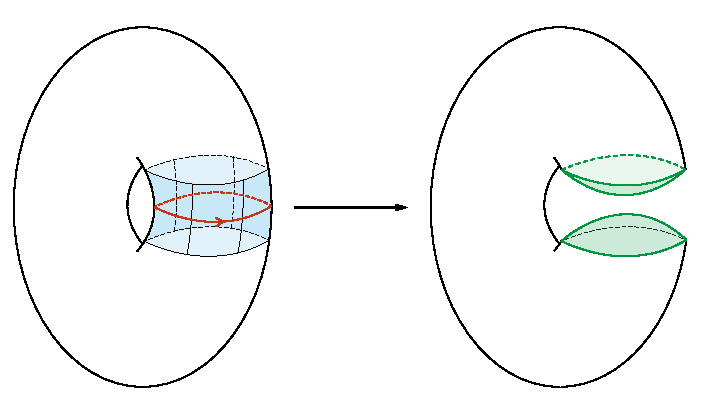
\includegraphics[scale=1]{graphics/surgery.pdf}
    \caption{Test}
\end{figure}

\begin{proposition}
    \label{appendix:prop:surger_killer}
    Let $W^n$ be a smooth manifold with basepoint $w_0 \in W$, $M \subseteq \partial W$ a subset of the boundary with basepoint $x_0 \in M$, $2(k+1) \leq n$ and $k \geq 1$.
    \begin{enumerate}[label=(\roman*)]
        \item \label{appendix:eq:surgery_killer_absolute_version} Let $\alpha_1,\ldots,\alpha_l \in \pi_k(W,w_0)$ be classes, which are represented by embeddings with trivial normal bundle. Then there exists a manifold $W^\prime$ obtained from $W$ by $l$-many $k$-surgeries away from the point $w_0$ together with a homomorphism $\phi \colon \pi_1(W,w_0) \to \pi_1(W^\prime,w_0)$ and a $\phi$-equivariant epimorphism
        \[
        \pi_k(W,w_0) \twoheadrightarrow \pi_k(W^\prime,w_0)
        \]
        containing $\alpha_1,\ldots,\alpha_l$ in its kernel. Moreover, 
        \[
        \pi_i(W,w_0) \cong \pi_i(W^\prime,w_0)
        \] 
        for all $i \leq k-1$.
        \item \label{appendix:eq:surgery_killer_relative_version} Let $\alpha_1^\mathrm{rel},\ldots,\alpha_l^\mathrm{rel} \in \pi_k(W,M,x_0)$ be classes, which lift to classes $\alpha_1,\ldots,\alpha_l \in \pi_k(W,x_0)$ under the map $\pi_k(W,x_0) \to \pi_k(W,M,x_0)$ induced by the inclusion. Again assume that $\alpha_1,\ldots,\alpha_l$ are represented by embeddings with trivial normal bundle. Then there exists a manifold $W^\prime$ obtained from $W$ by $l$-many $k$-surgeries together with a $\pi_1(M,x_0)$-equivariant epimorphism
        \[
        \pi_k(W,M,x_0) \twoheadrightarrow \pi_k(W^\prime,M,x_0)
        \]
        containing $\alpha_1^\mathrm{rel},\ldots,\alpha_l^\mathrm{rel}$ in its kernel. Moreover, 
        \[
        \pi_i(W,M,x_0) \cong \pi_i(W^\prime,M,x_0)
        \] 
        for all $1 \leq i \leq k-1$.
    \end{enumerate}
\end{proposition}

\begin{remark}
    If $\pi_k(W,w_0)$ is abelian (for example if $k \geq 2$) equivariance of the epimorphism $\pi_k(W,w_0) \twoheadrightarrow \pi_k(W^\prime,w_0)$ implies that it contains the entire $\Z[\pi_1(W,w_0)]$-module generated by $\alpha_1,\ldots,\alpha_l$ in its kernel. An analogous statement holds in the relative case. 
\end{remark}

\noindent In the proof of the Proposition we will make use of the following basic lemma. 

\begin{lemma}
    \label{appendix:lem:change_of_basepoint_homotopy_lemma}
    Let $X$ be a topological space and let $H \colon S^k \times [0,1] \to X$ be a homotopy from some map $f \colon S^k \to X$ to some map $g \colon S^k \to X$. Fix a basepoint $s_0 \in S^k$ and consider the path $\gamma(t) := H(s_0,t)$ from $x_0 := f(s_0)$ to $x_1 := g(s_0)$. Then the change of basepoint isomorphism
    \[
    b_\gamma \colon \pi_k(X,x_0) \to \pi_k(X,x_1)
    \]
    induced by $\gamma$ maps the class $[f]$ to the class $[g]$.
\end{lemma}

\needspace{5cm}

\begin{proof}
    Represent the classes $[f]$ and $[g]$ by maps $f^\prime \colon D^k \to X$ and $g^\prime \colon D^k \to X$, which are constant on the boundary. Let $H^\prime \colon D^k \times [0,1] \to X$ be the corresponding homotopy from $f^\prime$ to $g^\prime$, such that $H^\prime(S^{k-1},t) = \gamma(t)$. Then by $b_\gamma([f^\prime])$ is by definition represented by 
    \[
    D^k \to X, \quad y \mapsto 
    \begin{dcases}
        f^\prime(2y), & \norm{y} \leq \frac{1}{2},\\
        \gamma(2\norm{y}-1), & \norm{y} \geq \frac{1}{2}.
    \end{dcases}
    \] 
    This map is homotopic to $g^\prime$ relative $S^{k-1}$ by virtue of the following homotopy. 
    \[
    D^k \times [0,1] \to X, \quad y \mapsto 
    \begin{dcases}
        H^\prime\left(\frac{2}{1+t}y,t\right), & \norm{y} \leq \frac{1}{2}(1+t),\\
        \gamma(2\norm{y}-1), & \norm{y} \geq \frac{1}{2}(1+t).
    \end{dcases}
    \] 
\end{proof}

\begin{proof}[Proof of Proposition \ref{appendix:prop:surger_killer}]
    We first prove the absolute version \ref{psc:eq:surgery_killer_absolute_version} of the Proposition in three steps. \vspace{-.5em}

    \noindent \textbf{Step 1.} We start by explaining how to kill a single homotopy class by surgery. Suppose that $w_0 \in W$ is an interior point. Let $\beta \in \pi_k(W,w_0)$ be a class represented by an embedding $f \colon (S^k,s_0) \to (W,w_0)$ for a specified basepoint $s_0 \in S^k$, which extends to an embedding $F \colon S^k \times D^{n-k} \to W$ into the interior of $W$. Let 
    \begin{align*}
        \tilde{W} &:= W - \mathrm{int}(\mathrm{im}(F))
    \end{align*}
    and define $W^\prime$ by the pushout
    \[\begin{tikzcd}
	{S^k \times S^{n-k-1}} & {\tilde{W}} \\
	{D^{k+1} \times S^{n-k-1}} & {W^\prime}
	\arrow[from=1-1, to=1-2]
	\arrow[from=1-1, to=2-1]
	\arrow[from=1-2, to=2-2]
	\arrow[from=2-1, to=2-2]
    \end{tikzcd}\]
    as discussed above. Since the inclusion $S^k \times S^{n-k-1} \to D^{k+1} \times S^{n-k-1}$ is a cofibration it follows that the above suqare is a homotopy pushout, hence the map $\tilde{W} \to W^\prime$ has the same connectivity as $S^k \times S^{n-k-1} \to D^{k+1} \times S^{n-k-1}$, which is $k$-connected. Similiarly, the pushout 
    \[\begin{tikzcd}
	{S^k \times S^{n-k-1}} & {\tilde{W}} \\
	{S^k \times D^{n-k}} & W
	\arrow[from=1-1, to=1-2]
	\arrow[from=1-1, to=2-1]
	\arrow[from=1-2, to=2-2]
	\arrow[from=2-1, to=2-2]
    \end{tikzcd}\]
    implies that $\tilde{W} \to W$ is $n-k-1$-connected. Choose any point $d_0 \in \partial D^{n-k} = S^{n-k-1}$ and set $w_0^\prime := F(s_0,d_0)$. We now construct an epimorphism $\Psi_k \colon \pi_k(W,w_0) \to \pi_k(W^\prime,w_0^\prime)$ mapping the class $\beta$ to $0$. Choose a path $\lambda \colon [0,1] \to D^{n-k}$ from the center point $0 \in D^{n-k}$ to $d_0$ and let
    \[
    \eta(t) := F(s_0,\lambda(t)).
    \]
    Then $\eta$ is a path from $w_0$ to $w_0^\prime$ and we can consider the change of basepoint isomorphism
    \[
    b_\eta \colon \pi_k(W,w_0) \to \pi_k(W,w_0^\prime)
    \]
    induced by $\eta$. From the preceeding arguments it follows, that the map $\pi_i(\tilde{W},w_0^\prime) \to \pi_i(W,w_0^\prime)$ induced by the inclusion is an isomorphism for $i \leq k$, since $2(k+1) \leq n$. Thus we can define maps
    \[
    \Psi_i \colon \pi_i(W,w_0) \xrightarrow{b_\eta} \pi_i(W,w_0^\prime) \xleftarrow{\cong} \pi_i(\tilde{W},w_0^\prime) \to \pi_i(W^\prime,w_0^\prime).
    \]
    By the above discussion $\Psi_i$ is an isomorphism for $i \leq k-1$ and an epimorphism for $i = k$. We now show that $\Psi_k$ maps the class $\beta$ to $0$. Define
    \[
    \tilde{f} \colon (S^k,s_0) \to (W,w_0^\prime), \; y \mapsto F(y,d_0).
    \]
    Then $\tilde{f}$ is freely homotopic to $f$ via the homotopy $(y,t) \mapsto F(y,\lambda(t))$, so it follows from Lemma \ref{appendix:lem:change_of_basepoint_homotopy_lemma} that $b_\eta(\beta)$ is represented by $\tilde{f}$. Note that the image of $\tilde{f}$ lies in $\tilde{W}$ and thus $\Psi_k(\beta)$ is represented by
    \[
    (S^k,s_0) \to (W^\prime,w_0^\prime), \; y \mapsto \tilde{f}(y).
    \]
    This map factors as the following composition of inclusions
    \[
    S^k \to D^{k+1} \times \{d_0\} \to W^\prime,
    \]
    which is clearly contractible. Therefore $\Psi_k(\beta) = 0$. 
    % Note that all maps in the definition of $\Phi_k$ are compatible with the respective $\pi_1$-actions, hence the entire $\Z[\pi_1(W,w_0)]$-module generated by $\beta$ is contained in the kernel of $\Phi_k$. 
    \vspace{.5em}

    \noindent \textbf{Step 2.} Next we explain how to kill multiple homotopy classes at once. To this end assume that $W$ is connected. Let $\beta_i \in \pi_k(W,w_i)$ for interior points $w_i \in W$, $1 \leq i \leq l$. Again suppose that the $\beta_i$ can be represented by embeddings $f_i \colon (S^k,s_0) \to (W,w_i)$, which extend to embeddings $F_i \colon S^k \times D^{n-k} \to W$ into the interior of $W$. Moreover assume these embeddings to be disjoint, that is $\mathrm{im}(F_i) \cap \mathrm{im}(F_j) = \emptyset$ for $i \neq j$. This allows us to do surgery along all $F_i$ at once, i.e. we can define 
    \[
    \tilde{W} := W - \bigcup_{i=1,\ldots,l} \mathrm{int}(\mathrm{im}(F_i))
    \]
    and let $W^\prime$ be defined by the pushout 
    \[\begin{tikzcd}
	{\coprod_{i=1,\ldots,l} S^k \times S^{n-k-1}} & {\tilde{W}} \\
	{\coprod_{i=1,\ldots,l}D^{k+1} \times S^{n-k-1}} & {W^\prime}
	\arrow[from=1-1, to=1-2]
	\arrow[from=1-1, to=2-1]
	\arrow[from=1-2, to=2-2]
	\arrow[from=2-1, to=2-2]
    \end{tikzcd}\]
    In order to make sense of the statement, that we can kill all homotopy classes $\beta_i$ at once we would like to consider them as elements in the same group. To achieve this let $d_0 \in S^{n-k-1}$ and $\lambda \colon [0,1] \to D^{n-k}$ be as in Step 1 and set 
    \[
    w_i^\prime := F_i(s_0,d_0), \; \, \eta_i(t) := F_i(s_0,\lambda(t)).
    \]
    Moreover choose any point $v_0 \in \tilde{W}$ together with paths $\gamma_i^\prime \colon [0,1] \to \tilde{W}$ from $w_i^\prime \to v_0$. Such paths exist, since $W$ was assumed to be connected and removing (thickened) spheres of codimension at least $2$ preserves connectedness. Let 
    \[
    \gamma_i := \gamma_i^\prime \ast \eta_i \colon [0,1] \to W
    \]
    denote the composed path from $w_i$ to $v_0$ and consider the following commutative diagram for $j \leq k$.
    \[\begin{tikzcd}
	{\pi_j(W,v_0)} & {\pi_j(W,v_0)} & {\pi_j(\tilde{W},v_0)} & {\pi_j(W^\prime,v_0)} \\
	{\pi_j(W,w_i)} & {\pi_j(W,w_i^\prime)} & {\pi_j(\tilde{W},w_i^\prime)} & {\pi_j(W^\prime,w_i^\prime)}
	\arrow["{\mathrm{id}}", from=1-1, to=1-2]
	\arrow["\cong"', from=1-3, to=1-2]
	\arrow[from=1-3, to=1-4]
	\arrow["{b_{\gamma_i}}", "\cong"', from=2-1, to=1-1]
	\arrow["{b_{\eta_i}}", "\cong"', from=2-1, to=2-2]
	\arrow["{b_{\gamma^\prime_i}}", "\cong"', from=2-2, to=1-2]
	\arrow["{b_{\gamma^\prime_i}}", "\cong"', from=2-3, to=1-3]
	\arrow["\cong"', from=2-3, to=2-2]
	\arrow[from=2-3, to=2-4]
	\arrow["{b_{\gamma^\prime_i}}", "\cong"', from=2-4, to=1-4]
    \end{tikzcd}\]
    Denote the map defined as the top horizontal composition by 
    \[
    \Phi_j \colon \pi_j(W,v_0) \to \pi_j(W^\prime,v_0).
    \]
    The same arguments as in Step 1 show that $\Phi_j$ is an isomorphism for $j \leq k-1$ and an epimorphism for $j = k$. Moreover we have seen in Step 1, that for $j=k$, the class $\beta_i$ is contained in the kernel of the bottom horizontal composition, hence $b_{\gamma_i}(\beta_i)$ is also contained in the kernel of $\Phi_k$. Define
    \[
    \phi := \Phi_1 \colon \pi_1(W,v_0) \to \pi_1(W^\prime,v_0)
    \]
    and note that all maps in the definition of $\Phi_k$ are compatible with the respective $\pi_1$-actions, hence $\Phi_k$ is $\phi$-equivariant. \vspace{.5em}

    \noindent \textbf{Step 3.} Finally we show how to kill multiple homotopy classes as formulated in \ref{psc:eq:surgery_killer_absolute_version}. Let $g_i \colon (S^k,s_0) \to (W,w_0)$ be embeddings with trivial normal  bundle representing the class $\alpha_i$. By a general position argument we can find isotopies $H_i \colon S^k \times [0,1] \to W$ from $g_i$ to embeddings $f_i \colon S^k \to W-\{w_0\}$, such that $f_i(S^k) \cap f_j(S^k) = \emptyset$ for $i \neq j$. Moreover we may assume, that the image of $f_i$ is contained in the interior of $W$. Since the normal bundle of $g_i$ is trivial, the same holds for $f_i$. Therefore we can extend the $f_i$ to embeddings 
    \[
    F_i \colon S^k \times D^{n-k} \to W - \{w_0\}
    \]
    into the interior of $W$, such that $\mathrm{im}(F_i) \cap \mathrm{im}(F_j) = \emptyset$ for $i \neq j$. Now we are in the setting as in Step 2 for $w_i = f_i(s_0)$ and $\beta_i = [f_i] \in \pi_k(W,w_i)$. Define paths $\gamma_i(t) := H_i(s_0,1-t)$ from $w_i$ to $w_0$. Then $b_{\gamma_i}(\beta_i) = \alpha_i$ by Lemma \ref{appendix:lem:change_of_basepoint_homotopy_lemma}. We would like to apply Step 2 to $v_0 = w_0$, however the paths $\gamma_i$ are not of the same form as in Step 2 yet. Let us ignore this issue for a moment and see how Step 3 follows. Again let $W^\prime$ be the manifold obtained by surgery along $F_1 ,\ldots, F_l$ as before. Step 2 now yields a homomorphism $\phi \colon \pi_1(W,w_0) \to \pi_1(W^\prime,w_0)$ together with a $\phi$-equivariant epimorphism
    \[
    \Phi_k \colon \pi_k(W,w_0) \to \pi_k(W^\prime,w_0)
    \]
    containing the $b_{\gamma_i}(\beta_i) = \alpha_i$ in its kernel. Moreover, $\pi_j(W,w_0) \cong \pi_j(W^\prime,w_0)$ for $j \leq k-1$. 

    We now construct a homotopy to bring $\gamma_i$ into the desired form. Let $t_i := \mathrm{sup}\{t \in [0,1] \mid \gamma_i([0,t]) \subseteq \mathrm{im}(F_i)\}$ be the first time at which $\gamma_i$ exits $\mathrm{im}(F_i)$. For $t \in [0,t_i]$ we can then write $\gamma_i(t)$ in the form 
    \[
    \gamma_i(t) = F_i(\tilde{\sigma}_i(t), \tilde{\lambda}_i(t)).
    \]
    for suitable paths $\tilde{\sigma}_i, \tilde{\lambda}_i$. Now $\tilde{\sigma}_i$ and $\tilde{\lambda}_i$ are homotopic to the reparametrized paths 
    \[
    \begin{aligned}
    \sigma_i(t) = \begin{dcases}
    \tilde{\sigma}_i(0) = s_0, & t \in \left[0,\frac{t_i}{2}\right] \\
    \tilde{\sigma}_i(2t-t_i), & t \in \left[\frac{t_i}{2},t_i\right]
    \end{dcases} \text{ and }
    \qquad
    \lambda_i(t) = \begin{dcases}
    \tilde{\lambda}_i(2t), & t \in \left[0,\frac{t_i}{2}\right] \\
    \tilde{\lambda}_i(t_i), & t \in \left[\frac{t_i}{2},t_i\right]
    \end{dcases}
    \end{aligned}
    \]
    respectively. So after applying this homotopy we may replace $\tilde{\sigma}_i$ and $\tilde{\lambda}_i$ by $\sigma_i$ and $\lambda_i$. For $t \in  \left[0,\frac{t_i}{2}\right]$, $\gamma_i(t)$ can then be written as 
    \[
    \gamma_i(t) = F_i(s_0,\lambda_i(t)),
    \]
    which is of the same form as $\eta_i$ in Step 2. It remains to bring $\gamma^\prime_i := \gamma_i|_{\left[\frac{t_i}{2},1\right]}$ into the desired form, meaning the image of $\gamma_i^\prime$ should be completely contained within $\tilde{W}$. We can achieve this as follows. Applying a general position argument we can assume, that $\gamma_i^\prime$ does not intersect any of the embedded spheres $f_1(S^k), \ldots, f_l(S^k)$. Consider the deformation retraction
    \[
    r \colon W - \bigcup_{j=1,\ldots,l} f_j(S^k) \to \tilde{W}
    \]
    induced by the deformation retractions $S^k \times (D^{n-k} - 0) \to S^k \times S^{n-k-1}$. Then $r \circ \gamma_i^\prime$ is a path in $\tilde{W}$, which is homotopic to $\gamma_i^\prime$ relative to the endpoints. So in conlcusion we may indeed assume, that $\gamma_i$ is of the form as in Step 2.

    \vspace{.5em}

    \noindent \textbf{Step 4.} We can now deduce the relative version \ref{psc:eq:surgery_killer_relative_version} of the proposition using \ref{psc:eq:surgery_killer_absolute_version} applied to the given classes $\alpha_1, \ldots, \alpha_l \in \pi_k(W,x_0)$. Using these classes construct $\tilde{W}$ and $W^\prime$ as before. For $i \leq k$ consider the following diagram, where all maps are induced by inlcusions and the rows are exact. 
    \[\begin{tikzcd}
	{\pi_i(M,x_0)} & {\pi_i(W,x_0)} & {\pi_i(W,M,x_0)} & {\pi_{i-1}(M,x_0)} & {\pi_{i-1}(W,x_0)} \\
	{\pi_i(M,x_0)} & {\pi_i(\tilde{W},x_0)} & {\pi_i(\tilde{W},M,x_0)} & {\pi_{i-1}(M,x_0)} & {\pi_{i-1}(\tilde{W},x_0)} \\
	{\pi_i(M,x_0)} & {\pi_i(W^\prime,x_0)} & {\pi_i(W^\prime,M,x_0)} & {\pi_{i-1}(M,x_0)} & {\pi_{i-1}(W^\prime,x_0)}
	\arrow[from=1-1, to=1-2]
	\arrow[from=1-2, to=1-3]
	\arrow[from=1-3, to=1-4]
	\arrow[from=1-4, to=1-5]
	\arrow["{\mathrm{id}}"', from=2-1, to=1-1]
	\arrow[from=2-1, to=2-2]
	\arrow["{\mathrm{id}}", from=2-1, to=3-1]
	\arrow["\cong"', from=2-2, to=1-2]
	\arrow[from=2-2, to=2-3]
	\arrow[from=2-2, to=3-2]
	\arrow[from=2-3, to=1-3]
	\arrow[from=2-3, to=2-4]
	\arrow[from=2-3, to=3-3]
	\arrow["{\mathrm{id}}"', from=2-4, to=1-4]
	\arrow[from=2-4, to=2-5]
	\arrow["{\mathrm{id}}", from=2-4, to=3-4]
	\arrow["\cong"', from=2-5, to=1-5]
	\arrow["\cong", from=2-5, to=3-5]
	\arrow[from=3-1, to=3-2]
	\arrow[from=3-2, to=3-3]
	\arrow[from=3-3, to=3-4]
	\arrow[from=3-4, to=3-5]
    \end{tikzcd}\]
    It follows from the Five Lemma that 
    \[
    \pi_i(\tilde{W},M,x_0) \to \pi_i(W,M,x_0)
    \] 
    is an isomorphism and 
    \[
    \pi_i(\tilde{W},M,x_0) \to \pi_i(W^\prime,M,x_0)
    \] 
    is an isomorphism for $i \leq k-1$. This shows $\pi_i(W,M,x_0) \cong \pi_i(W^\prime,M,x_0)$ for $i \leq k-1$. If $i = k$ the map $\pi_k(\tilde{W},x_0) \to \pi_k(W^\prime,x_0)$ is surjective and a diagram chase shows that 
    \[
    \pi_k(\tilde{W},M,x_0) \to \pi_k(W^\prime,M,x_0)
    \] 
    is surjective as well. Thus we can define the epimorphism
    \[
    \Phi_\mathrm{rel} \colon \pi_k(W,M,x_0) \xleftarrow{\cong} \pi_k(\tilde{W},M,x_0) \to \pi_k(W^\prime,M,x_0).
    \]
    We have already seen that $\alpha_1,\ldots,\alpha_l$ are contained in the kernel of the map 
    \[
    \pi_k(W,x_0) \xleftarrow{\cong} \pi_k(\tilde{W},x_0) \to \pi_k(W^\prime,x_0).
    \]
    So commutativity of the above diagram implies 
    \[
    \Phi_\mathrm{rel}(\alpha_i^\mathrm{rel}) = 0.
    \]
    Note that all maps in the definition of $\Phi_\mathrm{rel}$ are $\pi_1(M,x_0)$-equivariant, such that the same holds for $\Phi_\mathrm{rel}$.
\end{proof}